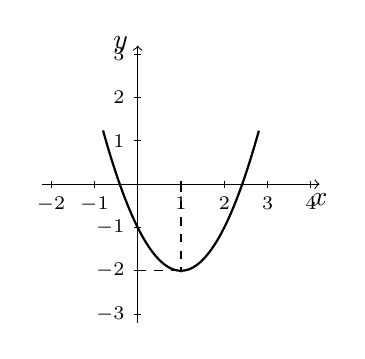
\begin{tikzpicture}[scale=0.55]
    \draw[->] (-2.2,0) -- (4.2,0) node[below] {$x$};
    \draw[->] (0,-3.2) -- (0,3.2) node[left] {$y$};
    \foreach \x in {-2,-1,1,2,3,4}
      \draw (\x,0.08)--(\x,-0.08) node[below] {\scriptsize $\x$};
    \foreach \y in {-3,-2,-1,1,2,3}
      \draw (0.08,\y)--(-0.08,\y) node[left] {\scriptsize $\y$};
    \draw[smooth, samples=200, domain=-0.8:2.8, thick] plot (\x, {(\x-1)^2-2});
    \fill (1,-2) circle (1.2pt);
    \draw[dashed] (1,0)--(1,-2);
    \draw[dashed] (0,-2)--(1,-2);
\end{tikzpicture}
